% \special{dvipdfmx:config z 0}
\documentclass[UTF8,a4paper,AutoFakeBold,AutoFakeSlant]{article}
\usepackage[a4paper,left=2.8cm,right=2.6cm,top=3.7cm,bottom=3.5cm]{geometry}
\usepackage{ctex}
% \usepackage{xeCJK}
\usepackage{graphicx}
\usepackage{pythonhighlight}
\usepackage[mathscr]{eucal}
\usepackage{mathrsfs}
\usepackage{booktabs}
\usepackage{capt-of} 
\usepackage{hyperref} 
\usepackage{abstract}
\usepackage{amsmath}
\usepackage{listings}
\usepackage{color}
\usepackage{caption}
\usepackage{subfigure}
\usepackage{enumerate}
\usepackage{amsfonts} 
\usepackage{CJK,CJKnumb}
\usepackage{float}
% \usepackage{gbt7714}
\usepackage{framed}
\usepackage{multirow}


\newcommand{\song}{\CJKfamily{song}}    % 宋体   (Windows自带simsun.ttf)
\newcommand{\fs}{\CJKfamily{fs}}        % 仿宋体 (Windows自带simfs.ttf)
\newcommand{\kai}{\CJKfamily{kai}}      % 楷体   (Windows自带simkai.ttf)
\newcommand{\hei}{\CJKfamily{hei}}      % 黑体   (Windows自带simhei.ttf)
\newcommand{\li}{\CJKfamily{li}}        % 隶书   (Windows自带simli.ttf) 
\newcommand{\ssong}{\CJKfamily{STSong}}

\xeCJKsetup{SlantFactor = 0.3}
% \xeCJKsetup{SlantFactor = -0.7}
\setCJKmainfont[BoldFont=SimHei, SlantedFont=KaiTi]{SimSun}



% -- 中文字体 --
%\setCJKmainfont{Microsoft YaHei}  % 微软雅黑
%\setCJKmainfont{YouYuan}  % 幼圆
%\setCJKmainfont{NSimSun}  % 新宋体
%\setCJKmainfont{KaiTi}    % 楷体
% \setCJKmainfont{SimSun}   % 宋体
%\setCJKmainfont{SimHei}   % 黑体
% \setCJKfamilyfont{hwsong}{STSong}
 
% -- 英文字体 --
% \setmainfont{Times New Roman}
% \setmainfont{DejaVu Sans}
% \setmainfont{Latin Modern Mono}
% \setmainfont{Consolas}
% \setmainfont{Courier New}


\usepackage{xcolor}  	%高亮使用的颜色
\definecolor{commentcolor}{RGB}{85,139,78}
\definecolor{stringcolor}{RGB}{206,145,108}
\definecolor{keywordcolor}{RGB}{34,34,250}
\definecolor{backcolor}{RGB}{220,220,220}

\usepackage{accsupp}	
\newcommand{\emptyaccsupp}[1]{\BeginAccSupp{ActualText={}}#1\EndAccSupp{}}

\usepackage{listings}
\lstset{						%高亮代码设置
	language=python, 					%Python语法高亮
	linewidth=0.95\linewidth,      		%列表list宽度
	%basicstyle=\ttfamily,				%tt无法显示空格
	commentstyle=\color{commentcolor},	%注释颜色
	keywordstyle=\color{keywordcolor},	%关键词颜色
	stringstyle=\color{stringcolor},	%字符串颜色
	%showspaces=true,					%显示空格
	numbers=left,						%行数显示在左侧
	numberstyle=\tiny\emptyaccsupp,		%行数数字格式
	numbersep=5pt,						%数字间隔
	frame=single,						%加框
	framerule=0.1pt,						%划线
	escapeinside=@@,					%逃逸标志
	emptylines=1,						%
	xleftmargin=3em,					%list左边距
	backgroundcolor=\color{backcolor},	%列表背景色
	tabsize=4,							%制表符长度为4个字符
	% gobble=4							%忽略每行代码前4个字符
}




\renewcommand{\abstractname}{}    % clear the title
\renewcommand{\absnamepos}{empty}
%去除摘要两边缩进
\makeatletter
  \renewenvironment{abstract}{%
      \if@twocolumn
        \subsection*{\abstractname}%
      \else
        \small
        \begin{center}%
          {\bfseries \abstractname\vspace{-.5em}\vspace{\z@}}%
        \end{center}%
      \fi}
      {}
  \makeatother
  \lstset{
    language=Matlab,
    keywords={break,case,catch,continue,else,elseif,end,for,function,
       global,if,otherwise,persistent,return,switch,try,while},
    basicstyle=\ttfamily,
    keywordstyle=\color{blue}\bfseries,
    commentstyle=\color{dkgreen},
    stringstyle=\color{dkpurple},
    backgroundcolor=\color{white},
    tabsize=4,
    showspaces=false,
    showstringspaces=false
 }

\title{\textbf{\textsf{{\textsf{LB3} \heiti{机器学习概论}}}}} 
\author{\ssong PB19151769~~~~~~马宇骁}
\date{}

% 去掉红框
\hypersetup{
colorlinks=true,
linkcolor=black
}

\begin{document}



\maketitle

\tableofcontents
\newpage


% ----------------------------------section----------------------------------------------


\section{实验要求}

\begin{enumerate}
  \item 完成决策树(回归树)的算法
  \item 完成 XGBoost 的算法
  \item 书写你的报告
\end{enumerate}

\begin{itemize}
  \item 禁止使用 sklearn 或者其他的机器学习库,你只被允许使用numpy, pandas, matplotlib, 和 Standard Library, 你需要从头开始编写这个项目。
  \item 你可以和其他同学讨论,但是你不可以剽窃代码,我们会用自动系统来确定你的程序的相似性,一旦被发现,你们两个都会得到这个项目的零分。
\end{itemize}


% ----------------------------------section----------------------------------------------


\section{实验原理}

\subsection{决策树(回归树)}

决策树是一种基本的分类与回归方法。决策树由结点(node)和有向边(diredcted edge)组成。结点有两种类型:内部结点(internal node)和叶结点(leaf node)。内部结点表示一个特征或属性,叶结点表示一个类别或者某个值。
用决策树做分类或回归任务时,从根节点开始,对样本的某一特征进行测试,根据测试结果,将样本分配到其子结点;这时,每一个子节点对应着该特征的一个取值。如此递归地对样本进行测试并分配,直至到达叶结点。

\subsubsection{理论解释}
假设X和Y分别为输入和输出变量,并且Y是连续变量,给定训练数据集:
$$ D = \{ (x_1,y_1),(x_2,y_2),\dots, (x_N,y_N) \} $$

一个回归树对应着输入空间(即特征空间)的一个划分以及在划分的单元上的输出值。假设已将输入空间划分为M个单元 
$ R_1, R_2,\dots, R_M $,并且在每个单元 $R_i$ 上有一个固定的输出值 $c_i$ ,于是回归树模型可以表示为:
\begin{equation*}
  f(x)=\sum_{i=1}^{M} c_{i} I\left(x \in R_{i}\right)
\end{equation*}

用平方误差 $\sum_{x_{i} \in R_{m}}\left(y_{i}-f\left(x_{i}\right)\right)^{2}$ 来表示回归树对于训练数据的预测误差,
用平方误差最小的准则求解每个单元上的最优输出值。
易知,单元 $R_i$ 上的 $c_i$ 的最优值 $\hat{c_i}$ 是$R_i$上的所有输入实例 $x_j$ 对应的输出 $y_j$ 的均值,即:
\begin{equation*}
  \hat{c_{i}}=\operatorname{ave}\left(y_{j} \mid x_{j} \in R_{i}\right)
\end{equation*}


\subsubsection{划分点}
CART回归树采用启发式的方法对输入空间进行划分,选择第j个变量
$x^{(j)}$和它取的值s,作为切分变量(splitting variable)和切分点(splitting point),并定义两个区域:
\begin{equation*}
  R_{1}(j, s)=\left\{x \mid x^{(j)} \leq s\right\} \text { 和 } R_{2}(j, s)=\left\{x \mid x^{(j)}>s\right\}
\end{equation*}

然后寻找最优切分变量j和最优切分点s。即求解:
\begin{equation*}
  \min _{j, s}\left[\min _{c_{1}} \sum_{x_{i} \in R_{1}(j, s)}\left(y_{i}-c_{1}\right)^{2}+\min _{c_{2}} \sum_{x_{2} \in R_{2}(j, s)}\left(y_{i}-c_{2}\right)^{2}\right]
\end{equation*}
对固定输入变量j可以找到最优切分点s。


\subsubsection{叶节点的输出值}
用选定的最优切分变量j和最优切分点s划分区域并决定相应的输出值:
\begin{equation*}
  \hat{c}_{1}=\operatorname{ave}\left(y_{i} \mid x_{i} \in R_{1}(j, s)\right) \text { 和 } \hat{c}_{2}=\operatorname{ave}\left(y_{i} \mid x_{i} \in R_{2}(j, s)\right)
\end{equation*}
遍历所有输入变量,找到最优的切分变量j,构成一个对(j, s)。依此将输入空间划分为两个区域。接着,对每个区域重复上述划分过程,直到满足停止条件为止。
对于已经划分输入空间好的,模型表示为:
\begin{equation*}
  f(x)=\sum_{i=1}^{M} \hat{c_{i}} I\left(x \in R_{i}\right)
\end{equation*}


\subsubsection{Obj}
\begin{equation*}
  O b j^{(t)}=\sum_{j=1}^{T}\left[G_{j} w_{j}+\frac{1}{2}\left(H_{j}+\lambda\right) w_{j}^{2}\right]+\gamma T
\end{equation*}

\begin{itemize}
  \item 权重
\end{itemize}

\begin{equation*}
    \frac{\partial O b j^{(t)}}{\partial w} = \sum_{j=1}^{T}\left[G_{j}+\left(H_{j}+\lambda\right) w_{j}\right] = 0
\end{equation*}
且对每一个$w_j$求偏导也等于0.

$ \Longrightarrow  $
\begin{equation*}
  w_j^* = -G_j(H_j+\lambda)^{-1}
\end{equation*}

\begin{itemize}
  \item Obj
\end{itemize}

\begin{equation*}
  \begin{aligned}
    {Obj^{(t)}}^* &= \sum_{j=1}^{T}\left[G_{j} {w_{j}^*}+\frac{1}{2}\left(H_{j}+\lambda\right) {w_{j}^*}^{2}\right]+\gamma T\\
    &= \sum_{j=1}^{T}\left[-G_{j}^2 (H_j+\lambda)^{-1}+\frac{1}{2} G_j^2 (H_j+\lambda)^{-1} \right]+\gamma T\\
    &= (\gamma - \frac{1}{2} G_j^2 (H_j+\lambda)^{-1})T
  \end{aligned}
\end{equation*}


\subsection{XGBoost}

基于boosting集成思想的加法模型,训练时采用前向分布算法进行贪婪的学习,每次迭代都学习一棵CART树来拟合之前 t-1 棵树的预测结果与训练样本真实值的残差。
XGBoost(eXtreme Gradient Boosting)极致梯度提升,是基于GBDT的一种算法。


\subsubsection{原理}
提升树模型可以表示为决策树的加法模型 :
$$ f_{M}(x)=\sum_{m=1}^{M} T_{m}(x) $$
其中,  $T_{m}(x)$  表示第  m  决策树,  M  为树的个数。


\subsubsection{初始化弱学习器}
\begin{equation*}
  f_{0}(x)=\arg \min _{c} \sum_{l=1}^{N} L\left(y_{i}, c\right)
\end{equation*}
假设取损失函数为平方损失。因为平方损失函数是一个凸函数,直接对  c  求导:
\begin{equation*}
  \sum_{i=1}^{N} \frac{\partial L\left(y_{i}, c\right)}{\partial c}=\sum_{i=1}^{N} \frac{\partial\left(\frac{1}{2}\left(y_{i}-c\right)^{2}\right)}{\partial c}=\sum_{i=1}^{N}\left(c-y_{i}\right)
\end{equation*}
等于0时,得 :
\begin{equation*}
  c=\sum_{i=1}^{N} y_{i} / N
\end{equation*}
所以初始化时,  c  取值为所有训练样本标签值的均值。此时得到初始学习器:
$f_{0}(x)=c$


\subsubsection{迭代训练}
对每个样本  i=1,2, $\cdots$, N  ,计算负梯度,即残差 :
\begin{equation*}
  r_{m i}=-\left[\frac{\partial L\left(y_{i}, f\left(x_{i}\right)\right)}{\partial f\left(x_{i}\right)}\right]_{f x)=f_{m-1}(x)}
\end{equation*}

将上步 得到的残差  $r_{m i}$  作为样本新的真实值,井将数据  $\left(x_{i}, r_{i m}\right), i=1,2, \cdots, N$  作为下 树的叶子结点的个数。

对  j=1,2, $\cdots$, J  个叶子结点,计算最佳拟合值:
\begin{equation*}
  c_{m j}=\arg \min _{c} \sum_{x_{i} \in R_{m j}} L\left(y_{i}, f_{m-1}\left(x_{i}\right)+c\right) \quad>c_{m j}
\end{equation*}

更新强学习器 :
\begin{equation*}
  f_{m}(x)=f_{m-1}(x)+\sum_{j=1}^{J} c_{m j} I\left(x \in R_{m j}\right)
\end{equation*}

最终的模型为:
\begin{equation*}
  \hat{f}(x)=f_{M}(x)=f_{0}(x)+\sum_{m=1}^{M} \sum_{j=1}^{J} c_{m j} I\left(x \in R_{m j}\right)
\end{equation*}




% ----------------------------------section----------------------------------------------


\section{实验实现}

事先将train.data文件改写成txt导入至excel文件中后读入。
\begin{quote}
  “在 train.data 文件中,有 7154 条 41 维的数据,其中前 40 列为 feature,最后一列为 label.”
\end{quote}

将数据随机打乱,9:1的比例划分训练集和测试集:
\begin{python}
  def split_train_test(data, test_ratio):
    np.random.seed(46)
    shuffled_indices = np.random.permutation(len(data))  # 生成和原数据等长的无序索引
    test_set_size = int(len(data) * test_ratio)
    test_indices = shuffled_indices[:test_set_size]
    train_indices = shuffled_indices[test_set_size:]
    return data.iloc[train_indices], data.iloc[test_indices]

  train,test = split_train_test(data, 0.1)
  train,test = train.to_numpy(),test.to_numpy()
  X_train,X_test = train[:,0:-1],test[:,0:-1]
  Y_train,Y_test = train[:,-1],test[:,-1]
\end{python}

\subsection{算法流程}

\subsubsection{决策树(回归树)}
输入:训练数据集$D$;

输出:回归树$f(x)$.

做如下步骤:
\begin{enumerate}
  \item 选择最优切分变量j与切分点s,即求解$$ \text{arg}\min _{j, s}\left[\min _{q_{1}} \sum_{x_{1} \in R_{1}(j, s)}\left(y_{i}-c_{1}\right)^{2}+\min _{c_{2}} \sum_{x_{1} \in R_{2}(j, s)}\left(y_{i}-c_{2}\right)^{2}\right] $$
  \item 用选定的对 (j, s) 划分区域并决定相应的输出值:$$ R_{1}(j, s)=\left\{x \mid x^{(j)} \leq s\right\}, \quad R_{2}(j, s)=\left\{x \mid x^{(j)}>s\right\} $$ $$ \hat{c}_{m}=\frac{1}{N_{m}} \sum_{x_{i} \in R_{m}(j, s)} y_{i}, \quad x \in R_{m}, \quad m=1,2 $$
  \item 对子区域递归调用1与2,直至满足停止条件(选择使用到最后一层停止)。
  \item 将输入空间划分为M个区域,生成决策树:$$ f(x)=\sum_{i=1}^{M} \hat{c_{i}} I\left(x \in R_{i}\right) $$
\end{enumerate}


\subsubsection{XGBoost}
输入: 训练数据集  $T=\left\{\left(x_{1}, y_{1}\right),\left(x_{2}, y_{2}\right), \cdots,\left(x_{n}, y_{n}\right)\right\} , x_{i} \in X \subseteq R^{n} , y_{i} \in Y \subseteq R$  ;

输出 : 提升树  $f_{M}(x)$

做如下步骤:
\begin{enumerate}
  \item 初始化  $f_{0}(x)=0 $
  \item 对  m=1,2, $\cdots$, M 
  \begin{enumerate}
    \item 计算残差 : $$ r_{m i}=y_{i}-f_{m-1}\left(x_{i}\right), \quad i=1,2, \cdots, N \quad $$
    \item 拟合残差 $ r_{m i}$  学习一个回归树, 得到  $T_{m}(x)$
    \item 更新  $f_{m}(x)=f_{m-1}(x)+T_{m}(x) $
  \end{enumerate}
  \item 得到:$$ f_{M}(x)=\sum_{m=1}^{M} T_{m}(x) $$
\end{enumerate}

\subsection{实验结果}

\subsubsection{决策树(回归树)}
取0-9十个不同的最大深度进行拟合训练,
训练曲线:
\begin{figure}[H]
  \centering
  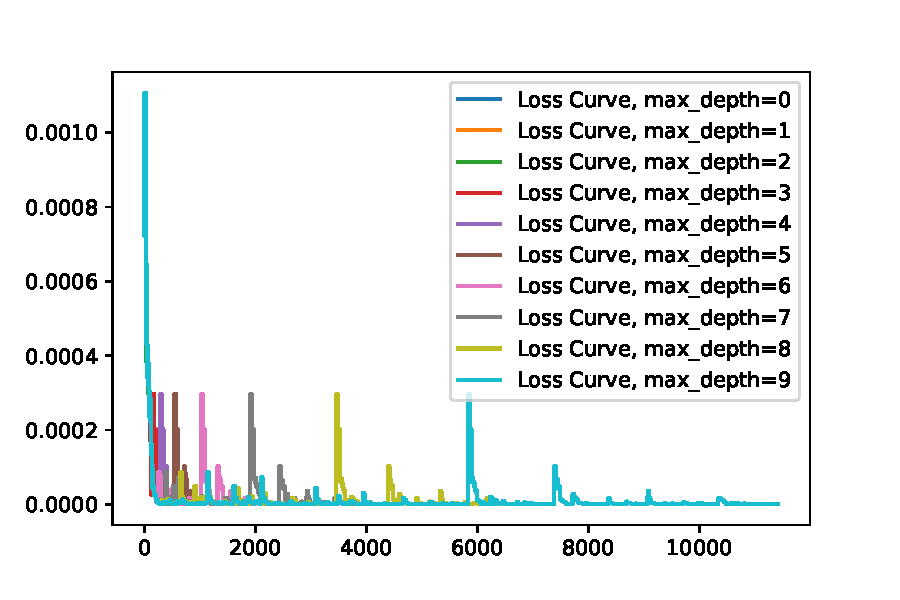
\includegraphics[scale=0.675]{loss.pdf}
  \caption{Loss Curve}
  \label{f1}
\end{figure}

对测试集预测,将RSS(也可以写做SSE)曲线绘制如下:
\begin{figure}[H]
  \centering
  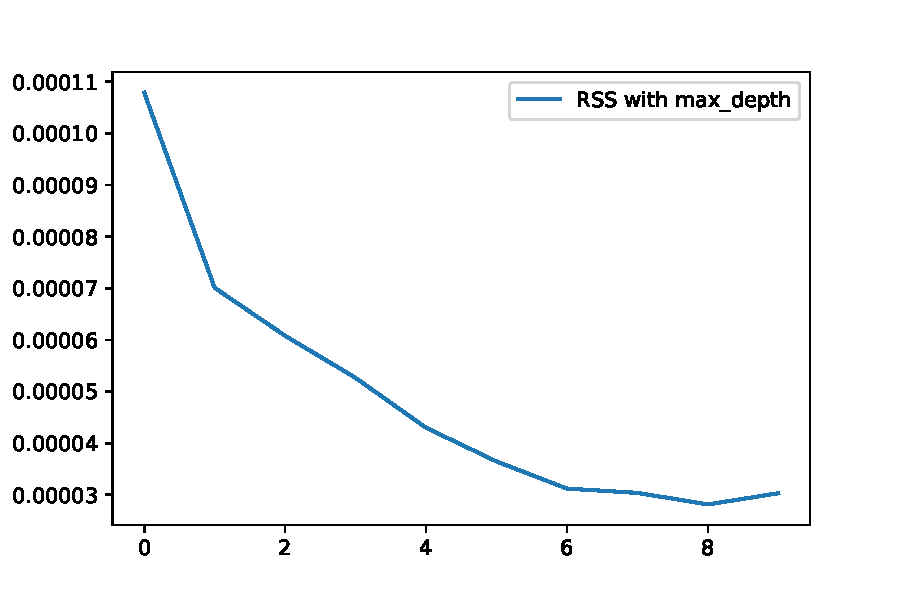
\includegraphics[scale=0.675]{rss.pdf}
  \caption{RSS}
  \label{f2}
\end{figure}

可以看出8的时候比较好。


\subsubsection{XGBoost}
展示1-5五个不同的最大深度进行拟合训练的
训练曲线:
\begin{figure}[H]
  \centering
  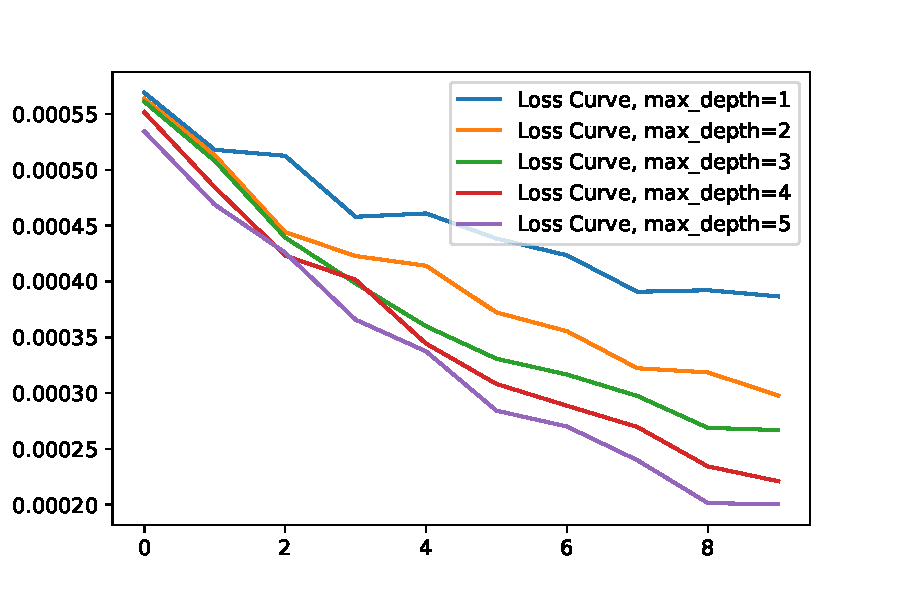
\includegraphics[scale=0.675]{boosting_treeloss.pdf}
  \caption{Loss Curve}
  \label{f3}
\end{figure}
这个比较明显的看出随着最大深度的增加损失下降明显。

对测试集预测,将RSS(1-14)曲线绘制如下:
\begin{figure}[H]
  \centering
  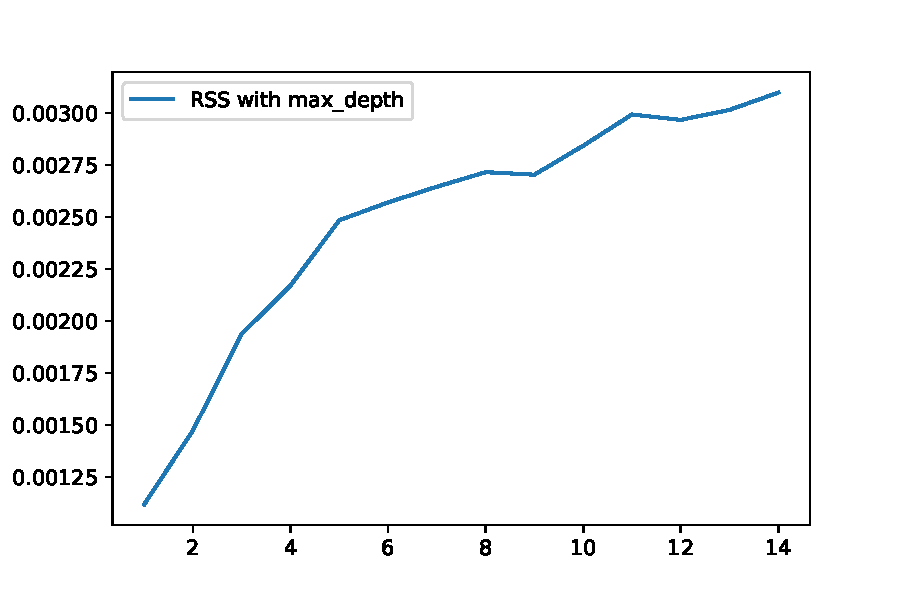
\includegraphics[scale=0.675]{boosting_treerss.pdf}
  \caption{RSS}
  \label{f4}
\end{figure}
发现误差并没有因为深度的增加而显著降低。





















% \bibliographystyle{gbt7714-numerical}
% % \bibliographystyle{7714-author-year}
% \bibliographystyle{ieeetr}
% \bibliography{bibl}

\end{document}